\documentclass[conference]{IEEEtran}
\IEEEoverridecommandlockouts
% The preceding line is only needed to identify funding in the first footnote. If that is unneeded, please comment it out.
\usepackage{cite}
\usepackage{amsmath,amssymb,amsfonts}
\usepackage{algorithmic}
\usepackage{graphicx}
\usepackage{textcomp}
\usepackage{xcolor}
\usepackage{listings}
\usepackage{mcode}
\usepackage{float}
\usepackage{amsmath}
\usepackage{longtable}
\usepackage{forest}


\newcommand{\abbrlabel}[1]{\makebox[2cm][l]{\textbf{#1}\ \dotfill}}
\newenvironment{abbreviations}{\begin{list}{}{\renewcommand{\makelabel}{\abbrlabel}}}{\end{list}}



\def\BibTeX{{\rm B\kern-.05em{\sc i\kern-.025em b}\kern-.08em
    T\kern-.1667em\lower.7ex\hbox{E}\kern-.125emX}}
    
    
\begin{document}

\title{Physio Denoise: A Model-based Tool for Modeling Physiological Noise in fMRI Data\\}

\author{\IEEEauthorblockN{Xinyi Wan KTH Royal Institute of Technology \\A Research Project in Stockholm University Brain Imaging Centre (SUBIC)}}

\maketitle

%\begin{abstract}
%\input{Chapters/Abstract}
%\end{abstract}

%\begin{IEEEkeywords}
%FMRI
%\end{IEEEkeywords}

\textit{Abbreviations}
\begin{abbreviations}
\item[MRI] Magnetic Resonance Imaging
\item[fMRI] Functional Magnetic Resonance Imaging
\item[BOLD] Blood-oxygen-level-dependent Signal  
\item[GLM] General Linear Model
\item[PPG] Photoplethysmogram 
\item[ROI] Region of Interest
\item[CSF] Cerebrospinal Fluid

\end{abbreviations}

\section{Introduction}\label{sec:Introduction}
Physiological noise is one of the significant artefacts in functional magnetic resonance imaging (fMRI).
fMRI uses magnetic imaging to measure brain activity by measuring changes in local oxygenation of blood, which in turn reflects the amount of local brain activity. \cite{poldrack2011handbook}
However, physiological pulsations related to cardiac pulsation and respiration would perturb blood-oxygen level contrast (BOLD) and add nuisance to fMRI data, which are the key challenges in this area. First, respiration is inevitable. 
During data aquisition, even the perfect subject could not avoid chest movement from breathing, which would result in head motion in the magnetic field. 
So that the MR images are likely to be distorted by respiration in a way.
Second, cardiac pulsation could directly influence the BOLD signal especially in the region with large blood vessels. 
For example, cerebrospinal fluid (CSF) flow is modulated by both the cardiac and respiratory cycles, resulting in additional signal changes.\cite{birn2012role}

The role of physiological noise in fMRI analysis deserves discussion. 
Some studies prefer not performing a physiological correction on fMRI data because cardiac and respiratory related fluctuations may be correlated with variations in neuronal activity.\cite{birn2012role} 
However, the spatial specificity of functional connectivity has been clearly demonstrated to be influenced by aliased physiological noise.\cite{lowe1998functional}
A functional connectivity study\cite{dagli1999localization} by Dagli has shown that removing cardiac fluctuations resulted in a variance reduction of roughly 10\%–40\%, 
depending on the region being investigated.\cite{dagli1999localization}
The sensitivity of these regions near pulsatile vessels could be improved by physiological noise correction. 
But another unarguable evidence is that heart rate variability is widely used as a measure of emotional arousal and autonomic nervous system activity.\cite{birn2012role} 
All these facts remind us that physiological noise correction shoule be used carefully especially when the key factors in experiments are related to physiological responses.

In this work, we provides a robust model-based tool XX in denoising physiological artefacts, which will give back a denoised data for further use. 
The implementation of this tool is based on the model RETROICOR.\cite{glover2000image}
This paper introduces the modules of this tool and explains results in each step from the example subject.

\section{Background}\label{sec:Background}
The goal of fMRI data analysis is to analyze each voxel's time series to see whether the BOLD signal changes in response to some manipulation \cite{poldrack2011handbook}.
And the method used for fMRI analysis in detection of signal changes is the general linear model(GLM). 
GLM, a well-developed tool of linear system analysis, is used widely to predict the responses of certain systems to a wide variety of inputs \cite{cohen1997parametric}.

In this work, our approach to addressing the problem of physiological artefacts is to record cardiac and respiratory signal during the scan, and then retrospectively remove these effects from the data \cite{glover2000image}.
GLM model is used as the basis of the denoise tool to build a noise model representing physiological artefact in fMRI images, and the cleaned data is obtained by regressing out physiological components in the model.

The general linear model could be expressed as:
\begin{equation}
\label{eqn:glm}
    Y = X\beta + e
\end{equation}
In the expression, $X$ is a design matrix containing linear variables for the model. And $Y$ is explained by the $X$ through weight $\beta$. And $\beta$ is the weight for each variable. The error of this model is estimated by $e$.

Inheriting the idea of GLM, noise model RETROICOR assumes that the signal could be expressed by additive noise components with weights. Both cardiac signal and respiration signal are regarded as periodic signals, 
so that they can be expressed as a low-Fourier series expanded in terms of these phases:
\begin{multline}
    Y(t) = \sum_{m = 1}^{M} a_m^c cos(m\phi_c) + b_m^c sin(m\phi_c) + \\ a_m^r cos(m\phi_r) + b_m^r sin(m\phi_r)
\end{multline}

In this expression, $\phi_c$ and $\phi_r$ are the phases in the respective cardiac and respiratory cycles. 
And the order of Fourier expression is configurable. In this work we used $M = 2$ as default.

For the calculation of cardiac phase, it is defined as
\begin{equation}
\label{eqn:cardiac}
    \phi_c(t) = 2\pi(t-t_1)/(t_2-t_1)
\end{equation}

Here $t_1$ and $t_2$ is the time for the subsequent R-peak value. 
So the expression constrains the phase value in the range from $0$ to $2\pi$. 
Since recorded physiological signals are used as inputs without any preprocessing, so R peak detection will be operated before the calculation.

For the calculation of respiratory phase, depth and states of breathing will be both taken into consideration. 
It is quite easy to imagine that a deeper breathe is more likely to bring a potential bulk motion of head. 
And also the phase of respiration is different from inhaling to exhaling. 
Therefore, respiratory phase is defined by both depth and state. 
State of inhaling or exhaling is more like polarity of phase, while depth is more like the amplitude value. 
The signal of depth is recorded by a detecting belt wrapping around subject's chest. 
To get the respiratory amplitude of the given time, a histogram-equalized transfer function is used, which is expressed  as :

\begin{equation}
    \phi_r(t) = \pi \frac{\sum_{b=1}^{rnd[R(t)/R_{max}]}H(b)}{\sum_{b=1}^{100}H(b)}dR/dt
\end{equation}

First, all the signal values are normalized to the range $(0, Rmax)$. Then a histogram $H(b)$ is gained with all normalized values. 
% In the $y$ domain of histogram, the $y$ value is from the normalized data. 
In the $x$ domain, the bins of histogram are defined to be 100 bins. 
If the normalized amplitude from the given time belongs to the $n$th bin, 
then the phase value will be calculated by dividing the sum value till $n$th bin by the sum of 100 bins.

In the end, value from the divisor will multiply by $\pi$, so that the phase value will be in the range from $-\pi$ to $\pi$.
During data acquisition of fMRI, BOLD time series have time resolution, which refers to repetition time or TR. 
And by now MRI data will be either recorded by multi-slice or single slice at a time, which means the slices that construct the whole brain volume come from different time stamp during the TR. 
Therefore, a single time stamp could not represent for the whole volume. 
However, applying different time stamps for each slice is also not practical. 
Because the slices are collected in horizontal direction, and the region of interest for artefacts could be in any shape rather than only scattering on a horizontal slice. 
So it is not meaningful to denoise slice by slice.
To simplify the slice time problem, the beginning time of each TR is chosen to calculate the physiological phases.

\section{Materials and methods}\label{sec:Methods}
\subsection{Overview}

\begin{figure*}
    \centering
    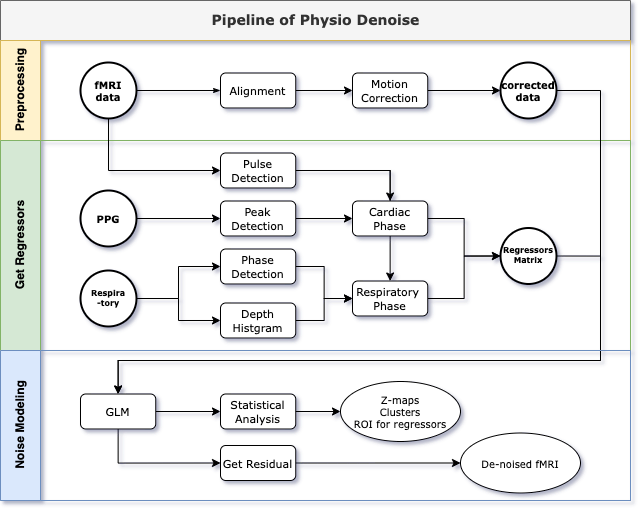
\includegraphics[width=0.8\textwidth]{Figures/pipe.png}
    \caption{Workflow of Physio Denoise}
    \label{fig:modules}
\end{figure*} 

Physio Denoise consists of three main modules, as depicted in Fig.\ref{fig:modules}, 
including preprocessing of fMRI data, preprocessing of physiological data  and noise modeling.
Briefly, the first modeule preprocesses the raw fMRI data with motion correction, 
and the second module deals with physiological data and generate the key values,
physiological regressors, from these data. 
These two modules prepare the basic materials for the noise modeling model. 
Exploiting the idea of RETROICOR model, 
noise modeling module uses prepared regressors to build a GLM.
Physiological regressors are used as independent variables in the model. 
So when regressing out all the physiological components, a cleaned fMRI data could be gained. 

The compulsory inputs for this tool include a raw fMRI data, 
physiological siganls saved in text file in which three columns respectively stand for cardiac signal, 
respiration signal and time stamps,
TR time, sample rate and working directory.

\subsection{Softwares and Packages}

(Introduction of needed toolds, to be continued.)

\textbf{FSL},

\textbf{Nilearn},


\textbf{HeartPy}\cite{van2019heartpy},

\textbf{Neurokit2}\cite{Makowski2021neurokit},

\textbf{Click},


\subsection{Data Preprocessing}

Although Physio Denoise is used for denoising, the preprocessing of fMRI data is still essential.
The preprcossing pipeline consists of alignment and motion correction.
% , as it shown in Fig.
% \ref{fig:graph}.

Alignment chooses the middle volume from the whole fMRI data as reference, and registers the other
volumes to it. 

The main idea of step motion correction is to correct the noise from motion noise. 
But different from the respiratory motion of breathing, this motion correction
is mainly bulk motion caused by subjects' movement. During the scan, motion noise is inevitable. 
Keeping subjects completely still during the whole scan is impractical.
Although small breaks are usually designed between each task during the scan in order to let subjects relax themselves, 
behaviours like swallowing and blinking exsist.
Bulk motion can have large effects on activation maps for analysis, 
which usually occur at edges in the image; 
this is due to the fact that large changes in image intensity can occur 
when a voxel that has no brain tissue in it at one point 
suddenly contains tissue due to motion.\cite{poldrack2011handbook}


% \begin{figure}[htp]
%     \centering
%     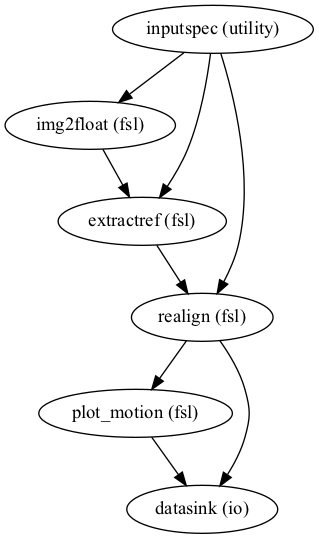
\includegraphics[width=0.7\columnwidth]{Figures/gragh.png}
%     \caption{The pipeline of preprocessing of fMRI data}
%     \label{fig:graph}
% \end{figure}

In order to model the physiological noise model more precisely, 
this step aims to clean the raw data roughly as the fisrt step.
Although in the whole motion noise, we still couldn't find a clear boundary
to seperate physiological noise and nosie from purely movement, a motion correction will
still help with the specificity in noise modeling. And the correction in 6 degree is plotted 
as results.

\subsection{Processing of Physiological data}
The main idea of processing physiological data is to extract needed regressors for the noise model.

\subsubsection{Scan Time Detection}
The whole denoising process aims at correcting fMRI data for each scan. 
So the time stamp of the beginning of each scan could be used to represent each volume image. 
Using scan time detection part also synchronizs physiological signals to each volume in fMRI data,
which is essential to get regressors in the modeling part.

Segmentation is also applied on input physiological data which
limits the length of signals to be consistent with fMRI data. Because during the data aquisition the physiological
data could be collected by external equipments such as Biopac rather than MRI device.
So length of signals may not be the same as fMRI data. Moreover, as mentioned in the background, the respiratory phase calculation 
partly depends on the a histogram of the amplitude during the whole scan. So a uncompatible length of 
respiratory signal might influences the phase values which indirectly effects the noise model. To be specific, 
a period of unexpected unstable signal could be accidently collected when subjects taking off the 
device, which may change the distribution of histogram in a way.

After scan time detection, the length of physiological signals will be limited to be 2 TR time longer than the 
fMRI data. And a csv file recording each scan time will be generated in the working directory.

\subsubsection{Cardiac Regressors}

In Physio Denoise, we choose a less invasive method of assess cardiac cycles, which is Photoplethysmogram (PPG). 
PPG devices employ an optical sensor to measure the changes in coloration of the skin as blood perfuses through the arteries and capillaries with each heartbeat.\cite{van2019heartpy}

With the help of HeartPy, the peak of the signal could be detected and marked, as it shows in Fig.\ref{fig:heart}

\begin{figure}[htp]
    \centering
    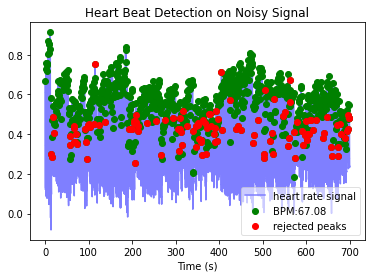
\includegraphics[width=\columnwidth]{Figures/heartpy.png}
    \caption{An example of PPG signal analyzed by HeartPy. The green points represent the accepted peaks,
    while the red points are rejected by HeartPy. Peaks are considered low confidence if the interval created between two adjacent peaks deviates 
    by more than 30\% of the mean peak-peak interval of the analysed segment.\cite{van2019heartpy}}
    \label{fig:heart}
\end{figure} 

\begin{figure}[htp]
    \centering
    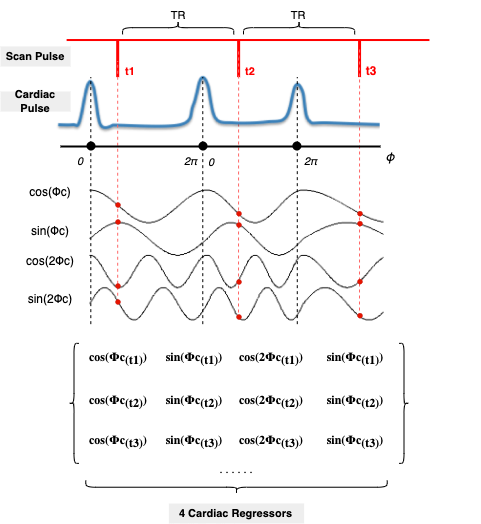
\includegraphics[width=\columnwidth]{Figures/cardiac.png}
    \caption{After detecting the peak in cardiac signal, the cardiac regressors from a second order Fourier expanded formula are generated with three MRI time stamps. 
    The matrix represents the way regressors constructing the independent variables $X$ in GLM }
    \label{fig:cardiac}
\end{figure} 

While a sequence of peaks from PPG signal is generated, 
two continous accepted peaks are found for the time stamp of each scan.
The scan time will locate between these two peaks. 
So that cardiac phase value in the formula \ref{eqn:cardiac} could be gained. An example of 
cardiac regressors calculation in Fig \ref{fig:cardiac} shows the process. 
In the design of GLM, each row of variable matrix in formula \ref{eqn:glm} indicates all used regressors
for one time stamp. The number of rows equals to the number of scan.

\subsubsection{Respiration Regressors}

Respiratory signal of subjects is collected by breathing belt, which warps around chest of subjects. 
So the belt would deform with expiration and inspiration, the amplitude of signal from the 
belt is recorded as respiratory signal. 

As we introduce before, respiratory phase calculation considers both breathing state and depth.
So in this part, it divides into two parts, state analysis and value calculation.

To analyze the state of breathing, a novel tool NeuroKit2\cite{Makowski2021neurokit} is exploited 
for detection. Inspiration, expiration and implausible periods are marked by NeuroKit2. 
Silmilar to the way of finding cardiac phase, with time stamps from MRI data, a respiratory phase
could be easily found with results from NeuroKit2. In Fig. \ref{fig:rsp_phase}, it shows part of the 
respiratory sample as well as the phases. The curve going down indicates the expiration, which 
phase value is $-1$. On the countary, a rising part represents inspiration with a phase value of $1$. 

\begin{figure}[htp]
    \centering
    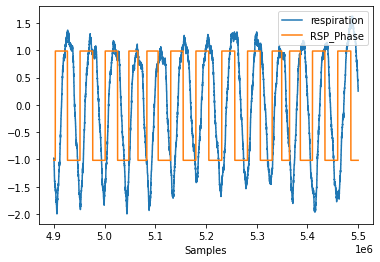
\includegraphics[width=\columnwidth]{Figures/rsp_phase.png}
    \caption{}
    \label{fig:rsp_phase}
\end{figure} 

To quantify the depth of breathe, a normalized histogram collecting all the amplitude values
shows a distribution of depth during the whole scan. 
So that at each given time stamp, its amplitude could locate the postion in histogram by the normalized value in x corordinate,
which is shown in the Fig.\ref{fig:hist}. For example, when the normalized amplitude is located in 
The value for respiratory phase is gained by dividing area A by the sum of area A and B.

\begin{figure}[htp]
    \centering
    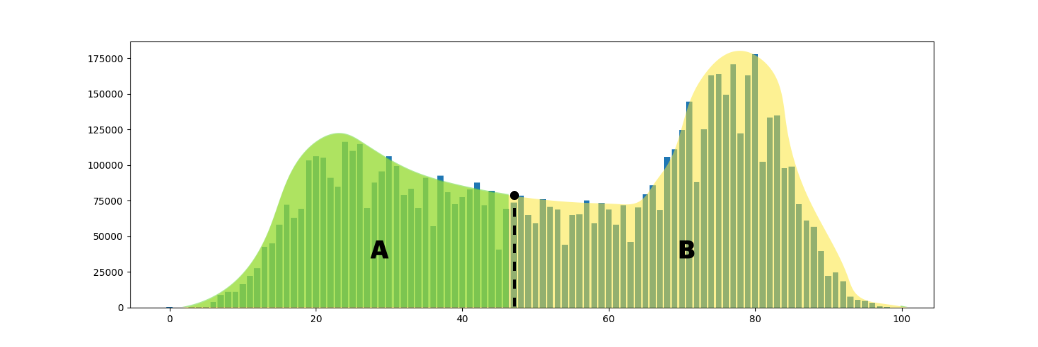
\includegraphics[width=\columnwidth]{Figures/histogram.png}
    \caption{}
    \label{fig:hist}
\end{figure}

However, the detection of breathing belt is based on physical motion that dosen't always give back
perfect data. Sometimes, the belt might be too loose or tight in measurement. The over tightness usually leads
to an abnormal amplitude that is higher than the normal range. In this work, abnormal signals will be 
kicked out before being used into the histogram.

Finally, phase value from the histogram will be given a polarity according to the state of the time.
Same as the cardiac regressors, each time stamp would have multiple regressors based 
on the Fourier expansion and its order.


\subsubsection{Noise Modeling}

Exploiting the idea of GLM, regressors from last step are independent variables in a GLM 
equation, while a preprocessed fMRI data is the dependent varaible. 
To find the region of interest(ROI) of different regressor, several contrasts are built and
each contrast represents one regressor. With the help of statistical analysis, 
Z-value maps from each contrast will show the specific region according to each regressor.
A z-map with a given threshold indicates the regions in which 
some noise signal is well expained by the according regressor.
In other words, it displays the region that physiological noise exsists. 
From the statistical analysis, the area of physiological noise is plotted for all regressors.
Moreover, clusters from GLM model with ROI are extracted. With the weight values from the results of GLM model, 
temporal signals are easily constructed for ROI as well as a frequency spectrum.

\subsection{Usage}

The usage of Physio Denois is straightfoward.


\section{Results}\label{sec:Results_And_Discussion}
\subsection{Sample Data}
Sample data used for showing the results by Physio Denoise includes 
resting state fMRI data, structural MRI data, PPG data and respiratory data.

The MRI data is aquired by Simens(XXX) with 1.7s of TR. Physiological data is aquired with Biopac(XXX) with 
sample frequency of 10000Hz.

\subsection{Results from Physio Denoise}
In three main steps of Physio Denoise, intermediate variables are also saved as outputs for analysis.
To simplify the output lists, the main outputs in each step from Physio Denoise are listed as below.
\\


\begin{forest}
    for tree={
      font=\ttfamily,
      grow'=0,
      child anchor=west,
      parent anchor=south,
      anchor=west,
      calign=first,
      edge path={
        \noexpand\path [draw, \forestoption{edge}]
        (!u.south west) +(7.5pt,0) |- node[fill,inner sep=1.25pt] {} (.child anchor)\forestoption{edge label};
      },
      before typesetting nodes={
        if n=1
          {insert before={[,phantom]}}
          {}
      },
      fit=band,
      before computing xy={l=15pt},
    }
  [Output directory
    [Step1 Preprocess
      [Display pipeline and dataflow]
      [motion correction
        [corrected data]
        [translation and rotations]
        ]
    ]
    [Step2 Regressors
      [detected scan pulse]
      [regressors]
      [respiration histogram]
    ]
    [Step3 Denoise
      [designed matrix]
      [Z-maps]
      [denoised data]
      [clusters and ROI]
    ]
  ]
\end{forest}

First, the z-maps from results of sample data are meaningful to inspect the ROI of physiological noise.
In Physio Denoise, a threshold of 2 is applied to all z-maps. And in default the order of Fourier
expasion is set to be $2$, which indicates 4 regressors for both cardiac and respiratory signals.

Here, results of sample data will show the ROI regions by Physio Denoise. In Fig.\ref{fig:zmap},
eight z-maps are showing the physiological noise related regions.

\begin{figure}[htp]
  \centering
  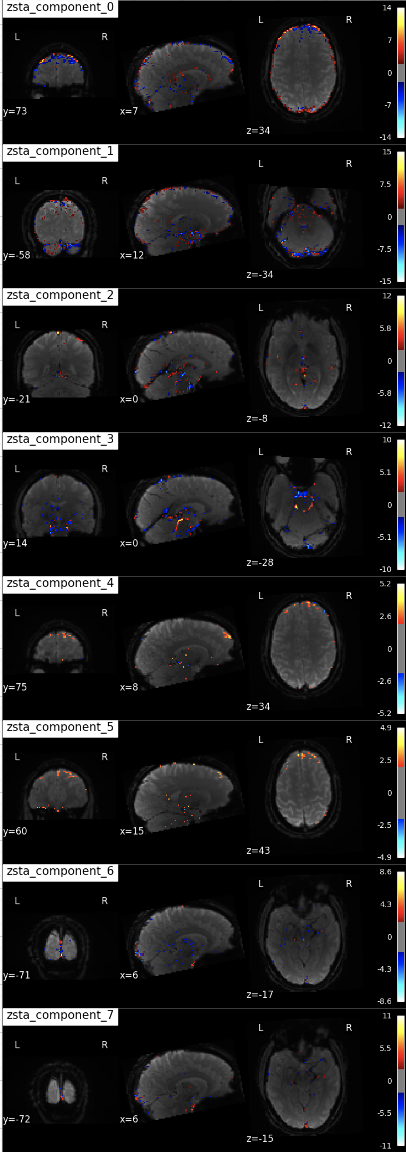
\includegraphics[width=0.9\columnwidth]{Figures/z-map.jpeg}
  \caption{Eight components from Z maps. Components 0-1: 1st order of respiration; Components 2-3: 1st order of cardiac;
  Components 4-5: 2nd order of respiration; Components 6-7: 2nd order of cardiac signal}
  \label{fig:zmap}
\end{figure} 

Component 0 and 1 come from the 1st order of Fourier expansion of respiratory signal.
From z-maps of component 0 and component 1, the highlight mainly loacates on the edge of skull. 
It indicates that the signals in the highlight part are hight correlated to respiratory signal. Moreover,
the signal on the edge of brain is less likely to be the neuronal signal. So that it is considered to be
the respiratory noise from fMRI.

Component 2 and 3 come from the 1st order of Fourier expansion of cardiac signal.
From z-maps of component 2 and 3, the highlight part mainly lies on the middle and back of the head.
Especially in the z-map of component 3, the highlight in the middle seems to be connected in a circle line, which is 
interpreted as circles of Willis. On the back of brain, the blood circulation in transverse sinus
could be reflected in z-map. A schematic diagram of veins in brain is shown in Fig.\ref{fig:brain}.

The components from the 2nd order are of less contrast in z-maps, but the regions of highlight
are silmilar to those of 1st order.

\begin{figure}[htp]
  \centering
  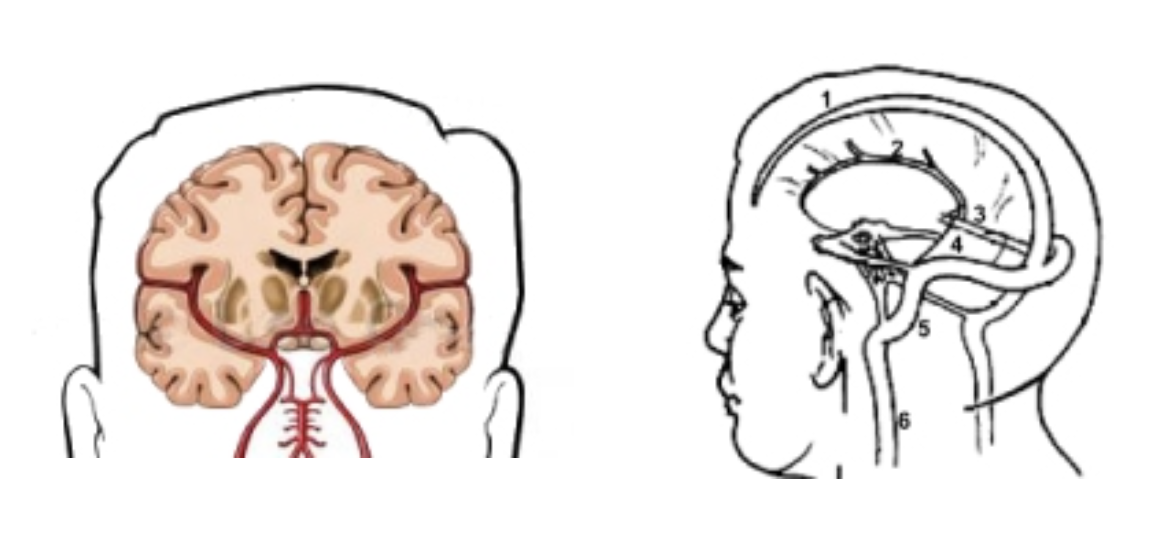
\includegraphics[width=0.9\columnwidth]{Figures/brain.jpeg}
  \caption{Structure of veins inside brain. 1. Superior sagittal sinus; 2. Inferior sagittal sinus;
  3. Straight sinus; 4. Transverse sinus; 5. Sigmoid sinus; 6. Internal jugular vein   }
  \label{fig:brain}
\end{figure} 






%\section{Analysis}\label{sec:Analysis}
%\input{Chapters/Analysis}

\section{Discussion}\label{sec:Discussion}
Physio Denoise is a robust denoising tool for fMRI data. 
Proceeding the raw txt file of physiological data with advanced bio-signal detecting tools, 
Physio Denoise could calculate the regressors for RETROICOR model directly.
In the meanwhile, Physio Denoise has strong visualization in outputs.
Important figures in the main step are generated for users to better understand the process.
And intermediate variables are able to trace back the calculating process.
In the results, all the noise components of high contrast 
are shown in the background of a structural brain image, which
is easy to relate brain structure to the possible reasons for explaining the noise.
The spectrum of predicted noise could also be used to analyze noise in frequency domain.

However, there are still several crucial problems and concern with Physio Denoise.

First, the whole implementation of Physio Noise is based on RETROICOR model and GLM. 
The nuisance regressors in the noise model are not completely linear independent 
and may exhibit shared variance \cite{bright2017potential}.
Those correlated regressors might 
add more difficulty to interpreting the influence from each component.
One possible solution to this problem is to include additional combined regressors into the model
from both respiratory and cardiac signals. Then the influence from correlated regressors 
could be taken into consideration. 

As mentioned previously, another related problem about the potential correlation 
between nuisance regressors and real neuronal events. 
Cardiac pulsation results in brain tissue movement and 
inflow effects leading to correlated signal fluctuations primarily 
in and near large blood vessels \cite{dagli1999localization}. The movement of the chest wall during breathing results 
in magnetic field changes that distort the MR image acquired of the brain \cite{brosch2002simulation}.
Moreover, Cerebrospinal fluid (CSF) inside brain will be manipulated by both respiration and cardiac cycles.

The concern with design of Physio Denoise is applying regressors to the entire brain. 
Apparently, physiological influence cannot be removed by the use of a single nuisance regressor 
for the entire brain (such as global signal regression) due to the 
clear regional heterogeneity of the physiologically-coupled responses. \cite{chen2020resting}
Step like regional division could be applied to the data before regression, which could lead to more precise
denoising.



% \section{Sustainability and ethics}\label{sec:Sust-Ethics}
% \input{Chapters/Sust-Ethics}

\section{Future Work}\label{sec:Future_Work}
The validity of Physio Denoise need to be examined in the future work.
One way to execute this essential work is to compare the results with others from existing tools.
The preliminary idea is applying different physiologically denoising tools to the raw data.
Several typical ROIs are chosen to compare the predicted noise signal, raw signal and denoised signal.
The performance of different noise models, such as
the variance, Signal-to-noise ratio(SNR) and R-Squared, will be used as main criteria.

% \section*{Contributions}\label{sec:Contributions}
% \input{Chapters/Contribution}

% References
\bibliographystyle{IEEEtran}
\bibliography{IEEEabrv,References}


%\newpage
%\onecolumn
%\input{Chapters/Appendix}
\end{document}